\begin{frame}
  \frametitle{Simple vs. complex settings - QITL-01 revisited}

  \begin{itemize}

  \item  Arppe \& J{\"a}rvikivi (2002, 2007)

  \item \textit{Person} (FIRST PERSON SINGULAR or not) and
    \textit{Countability} (COLLECTIVE or not) of AGENT/SUBJECT of
    Finnish verb synonym pair \textit{mietti{\"a}} vs. \textit{pohtia}
    'think, ponder': \\

{\tiny
\begin{table}[h]
\begin{tabular}{ c  c || c || c  c}
\hline
Forced-choice                         &                 & Frequency           &                                       & Acceptability    \\
Dispreferred                          & Preferred       & (relative)          & Unacceptable                          & Acceptable       \\ \hline \hline
\multicolumn{1}{c|}{$\varnothing$}    & mietti{\"a}+SG1 & Frequent            & \multicolumn{1}{c|}{$\varnothing$}    & mietti{\"a}+SG1  \\
\multicolumn{1}{c|}{}                 & pohtia+COLL     &                     & \multicolumn{1}{c|}{}                 & pohtia{\"a}+COLL \\ \hline
\multicolumn{1}{c|}{mietti{\"a}+COLL} &                 &                     & \multicolumn{1}{c|}{}                 &                  \\
\multicolumn{1}{c|}{pohtia+SG1}       & $\varnothing$   & Rare                & \multicolumn{1}{c|}{mietti{\"a}+COLL} & pohtia+SG1       \\
\hline
\end{tabular}
\end{table}
}

  \end{itemize}
\end{frame}

\begin{frame}[c]
  \frametitle{QITL-1 through the lenses of NDL: 1/4}

  \centering
  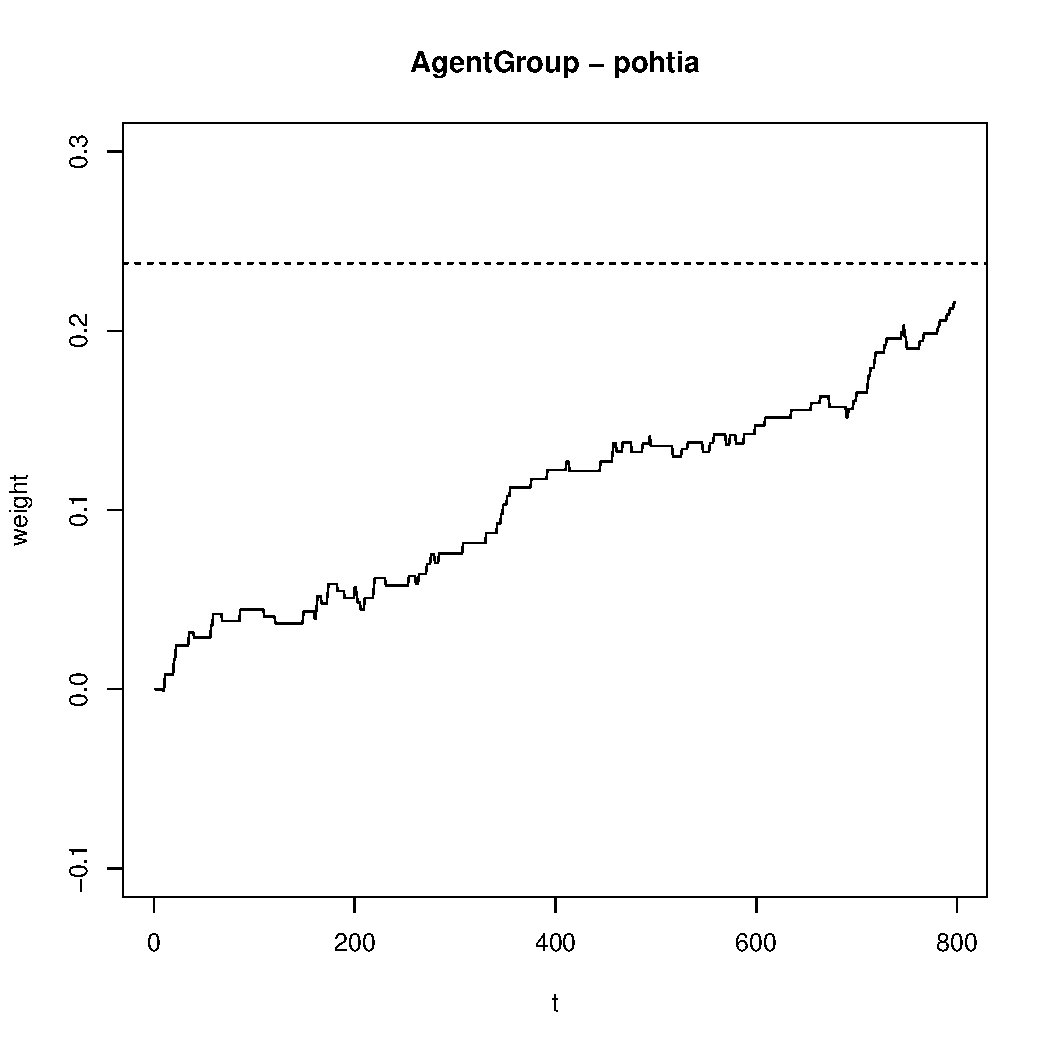
\includegraphics[width=8cm]{{{img/think.qitl1.AgentGroup_pohtia_RW_vs_D}}}
\end{frame}

\begin{frame}[c]
  \frametitle{QITL-1 through the lenses of NDL: 2/4}

  \centering
  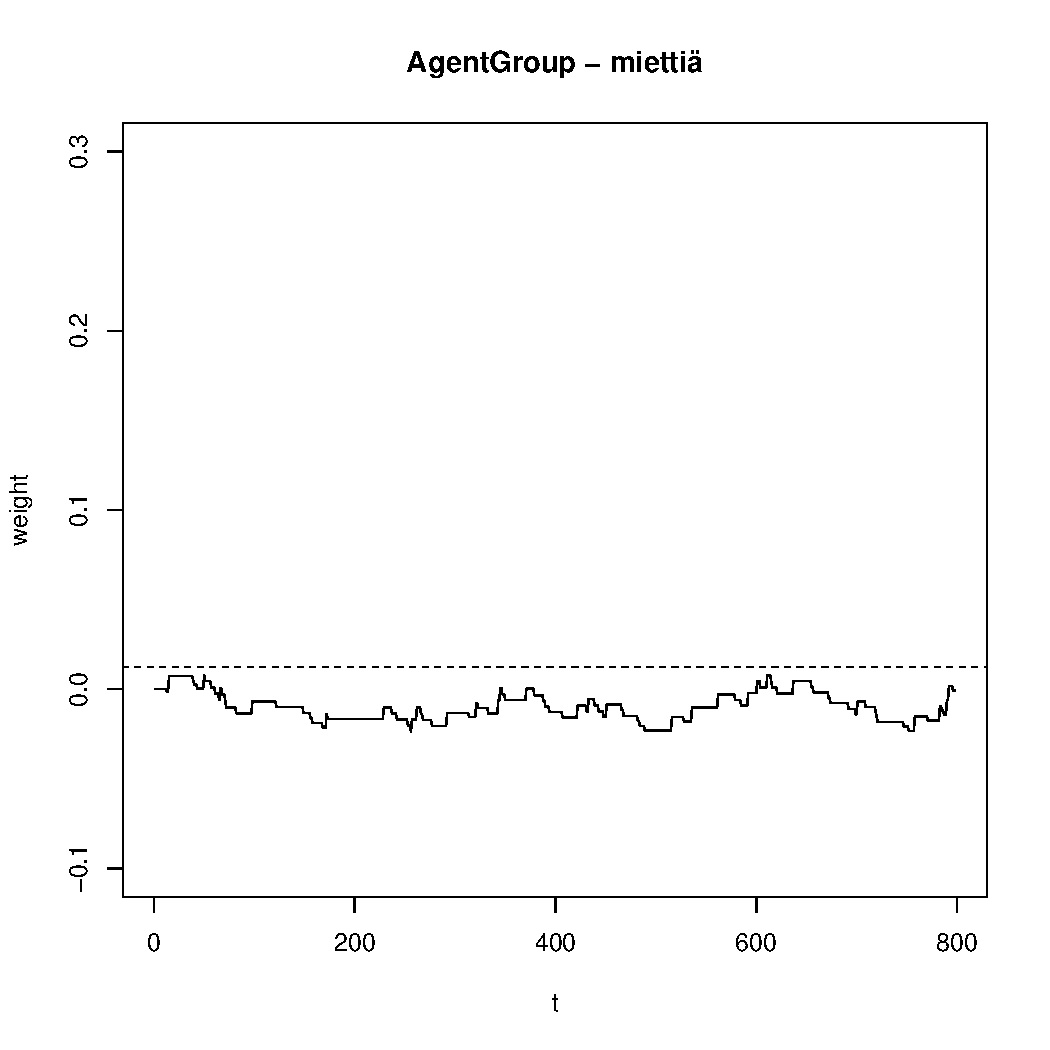
\includegraphics[width=8cm]{{{img/think.qitl1.AgentGroup_miettia_RW_vs_D}}}
\end{frame}

\begin{frame}[c]
  \frametitle{QITL-1 through the lenses of NDL: 3/4}

  \centering
  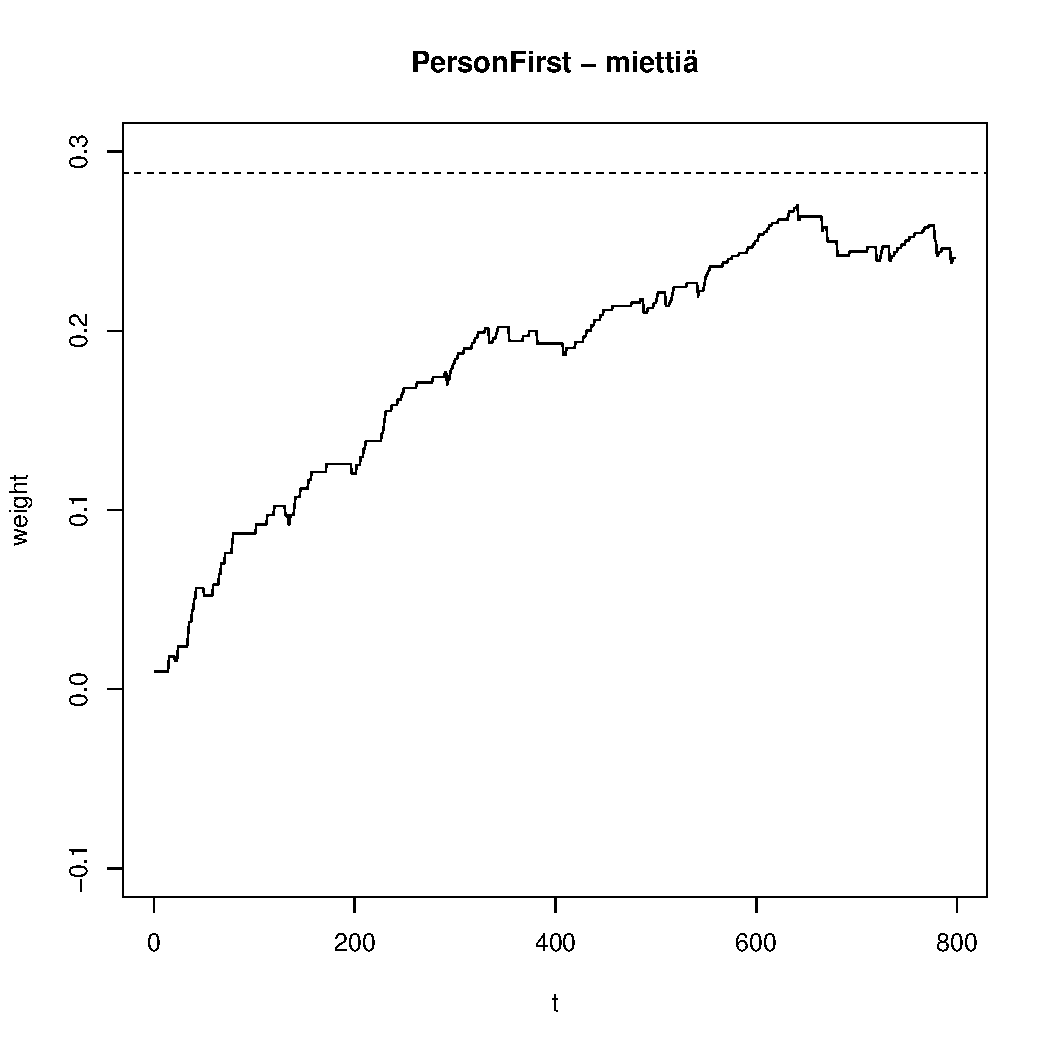
\includegraphics[width=8cm]{{{img/think.qitl1.PersonFirst_miettia_RW_vs_D}}}
\end{frame}


\begin{frame}[c]
  \frametitle{QITL-1 through the lenses of NDL: 4/4}

  \centering
  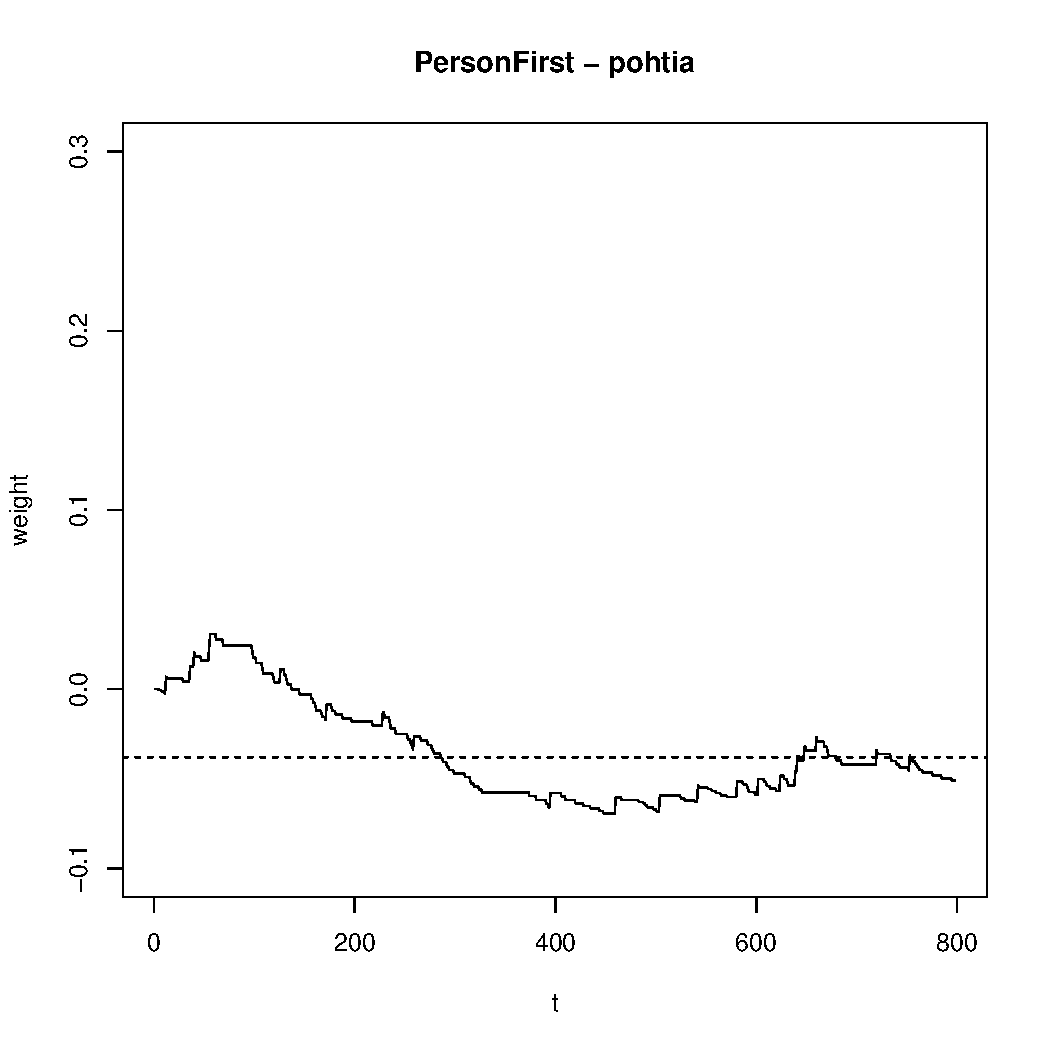
\includegraphics[width=8cm]{{{img/think.qitl1.PersonFirst_pohtia_RW_vs_D}}}
\end{frame}

\begin{frame}[c]
  \frametitle{QITL-01 through the lenses of QITL-6}
  \framesubtitle{(courtesy of Dagmar Divjak)}

  \centering
  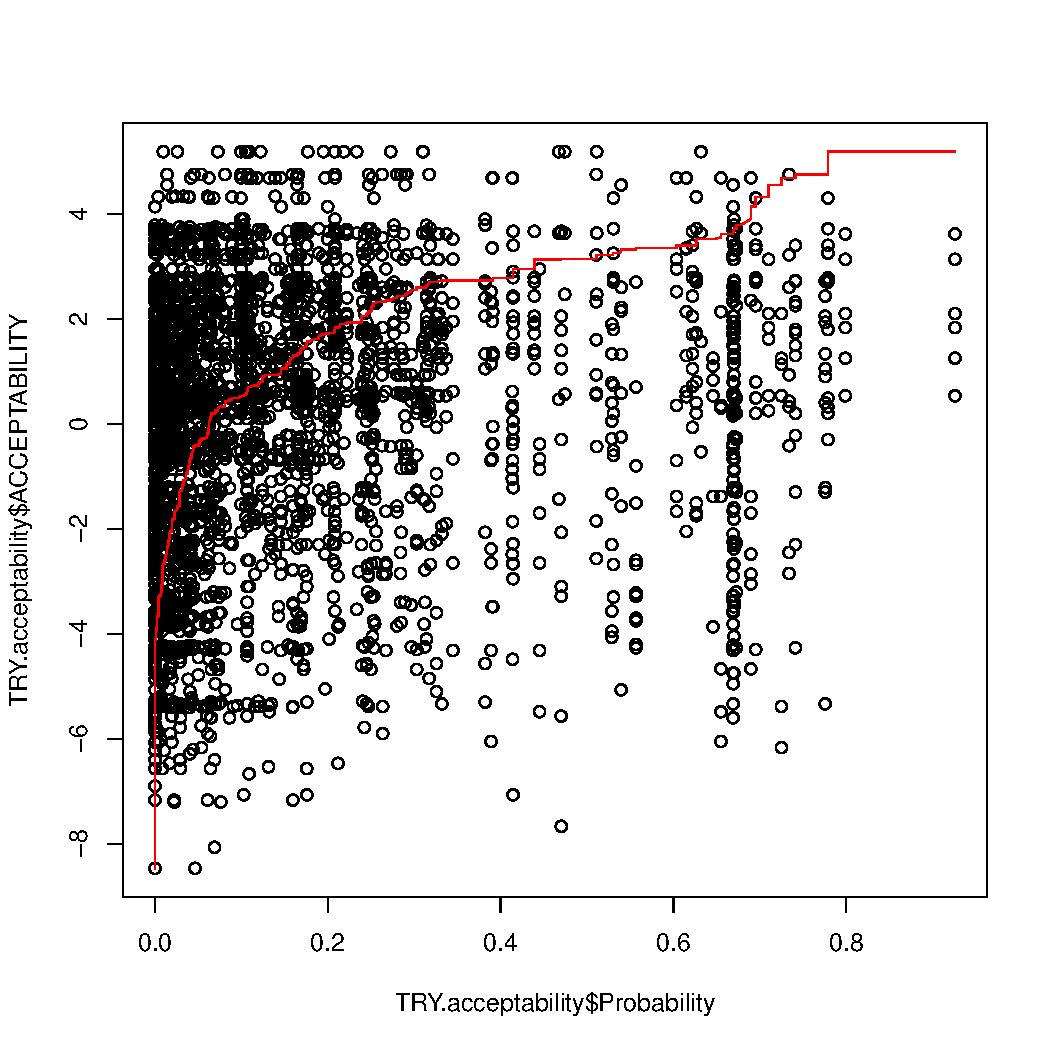
\includegraphics[width=7cm]{{{img/TRY.ACCEPTABILITY_vs_Probability}}}
\end{frame}

\begin{frame}[c]
  \frametitle{Simple vs. complex settings -- QITL-2 revisited}

  \centering
  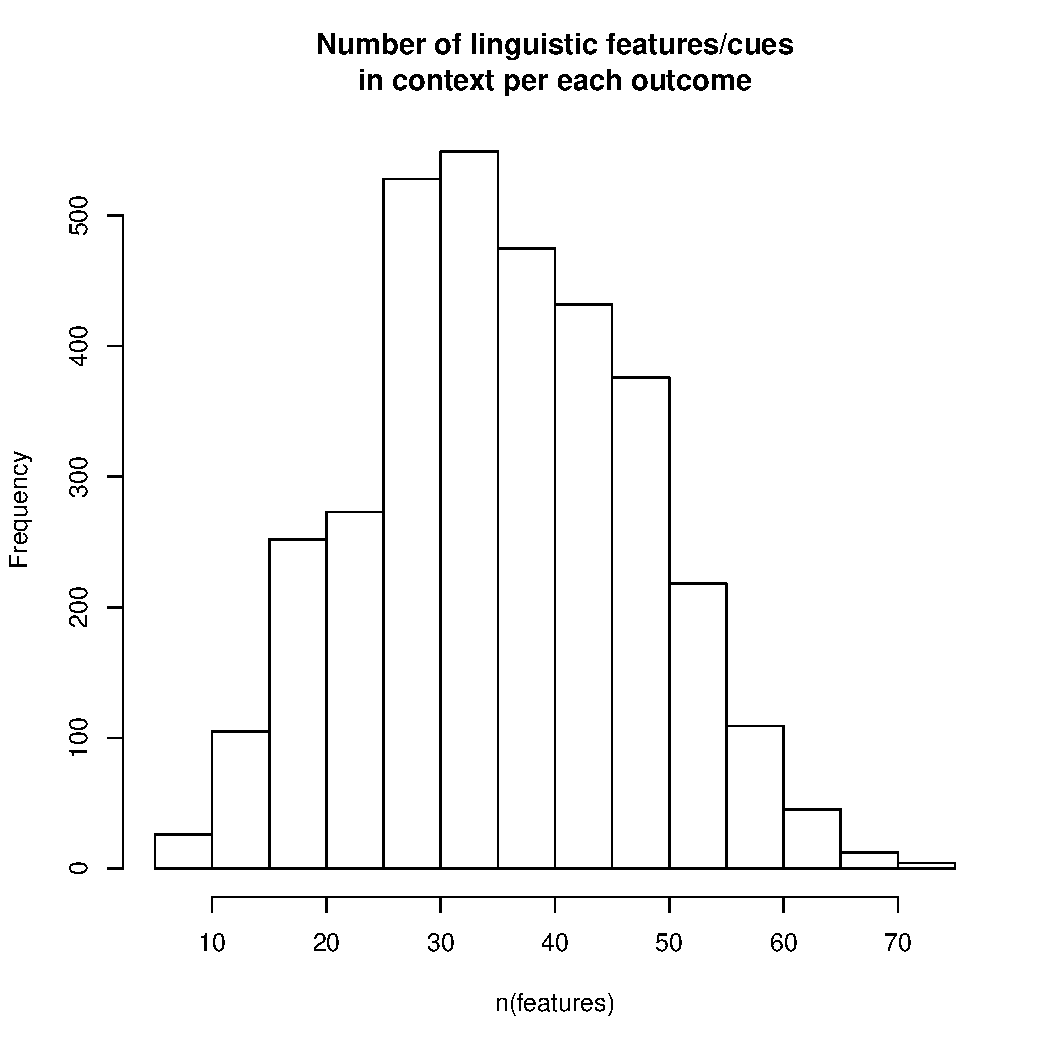
\includegraphics[width=8cm]{{{img/THINK.maximal_linguistic_variable_density}}}
\end{frame}

\begin{frame}
\frametitle{QITL-4 revisited -- comparison of NDL with statistical methods -- Classification Accuracy \& Recall}

% latex table generated in R 2.12.2 by xtable 1.5-6 package
% Fri May  6 00:15:47 2011
\begin{table}[ht]
  \begin{center}
    {\footnotesize
      \begin{tabular}{lrrr}
        \hline
        & $\lambda_{\mbox{\tiny prediction}}$ & $\tau_{\mbox{\tiny classification}}$ & Accuracy \\
        \hline
        Polytomous logistic regression & 0.368 & 0.488 & 0.645 \\
        (One-vs-rest) &  &  &  \\
        Polytomous mixed logistic regression &  &  &  \\
        (Poisson reformulation) &  &  &  \\
        1|Section & 0.360 & 0.482 & 0.640 \\
        1|Author & 0.358 & 0.481 & 0.640 \\
        1|Section + 1|Author & 0.358 & 0.481 & 0.640 \\
        Support Vector Machine & 0.340 & 0.466 & 0.629 \\
        Memory-Based Learning & 0.286 & 0.422 & 0.599 \\
        (TiMBL) &  &  &  \\
        Random Forests & 0.326 & 0.455 & 0.621 \\
        Naive Discriminative Learning & 0.346 & 0.471 & 0.632 \\
        \hline
      \end{tabular}
    }
    \caption{Classification diagnostics for five models fitted to the Finnish data set ($n=3404$).}
    \label{tab:results}
  \end{center}
\end{table}

\end{frame}

%%% Local Variables: 
%%% mode: latex
%%% TeX-master: "../qitl6_evert_arppe"
%%% End: 
